%%%%%%%%%%%%%%%%%%%%%%
%%%%%%%%%%%%%%%%%%%%%%
%%Options for presentations (in-class) and handouts (e.g. print). 
\documentclass[pdf
,handout
]{beamer}
\usepackage{pgfpages}
\pgfpagesuselayout{2 on 1}[letterpaper,border shrink=5mm]

\graphicspath{{../}}
%%%%%%%%%%%%%%%%%%%%%%
%% Change this for different slides so it appears in bar
\usepackage{authoraftertitle}
\date{Linear Transformations}

%%%%%%%%%%%%%%%%%%%%%%
%% Upload common style file
\usepackage{../LyryxLinearAlgebraSlidesStyle}

\begin{document}
	
	%%%%%%%%%%%%%%%%%%%%%%%
	%% Title Page and Copyright Common to All Slides
	
	%Title Page
	\input ../frontmatter/titlepage.tex
	
	%LOTS Page
	%\input frontmatter/lyryxopentexts.tex
	
	%Copyright Page
	\input ../frontmatter/copyright.tex
	
	%%%%%%%%%%%%%%%%%%%%%%%%%


\section{Introduction}
%-------------- start slide -------------------------------%
\frame{
\begin{block}{Notation and Terminology}
\pause 
\begin{itemize}
\item We have already used \alert{$\RR$} to denote the set 
of \alert{real numbers}.
\pause 
\item We use \alert{$\RR^2$} to the denote the set of
all \alert{column vectors of length two},
\pause
 and we use
\alert{$\RR^3$} to the denote the set of
all \alert{column vectors of length three}
\pause
\textcolor{blue}{(the length of a vector is the number
of entries it contains).}
\pause
\item In general, we write \alert{$\RR^n$} for the
set of all \alert{column vectors of length $n$}.
\end{itemize}
\end{block}
\pause
\begin{alertblock}{$\RR^2$ and $\RR^3$}
Vectors in $\RR^2$ and $\RR^3$ have convenient geometric
interpretations as {\bf position vectors} of points in
the 2-dimensional (Cartesian) plane and in 3-dimensional
space, respectively.
\end{alertblock}
}
%-------------- end slide -------------------------------%

%-------------- start slide -------------------------------%
\frame{%\frametitle{Geometric Vectors in $\RR^2$ and $\RR^3$}
\begin{picture}(4,2.5)
\put(0.3,0.7){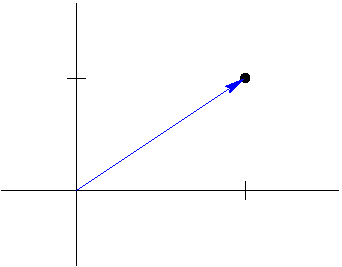
\includegraphics[scale=0.7]{figures/R2.pdf}}
\put(0.2,2.2){{$\RR^2$}}
\put(0.5,0.9){\scriptsize{$0$}}
\put(1.7,0.95){\scriptsize{$x$}}
\put(1.4,0.9){\scriptsize{$a$}}
\put(0.55,1.9){\scriptsize{$y$}}
\put(0.5,1.55){\scriptsize{$b$}}
\put(1.5,1.6){\scriptsize{\alert{$(a,b)$}}}
\pause
\put(0.5,0.3){\scriptsize\textcolor{blue}{The vector 
$\left[\begin{array}{c} a \\ b\end{array}\right]$.}} 
\pause
\put(2.4,2.4){{$\RR^3$}}
\put(2.5,0.3){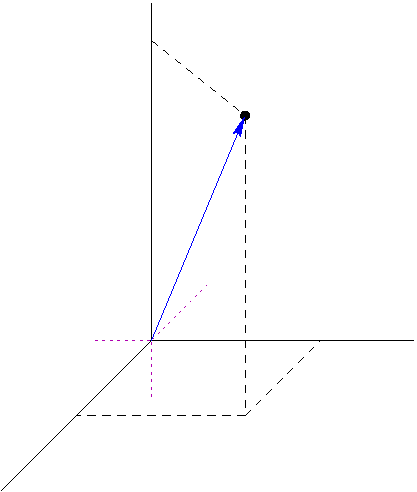
\includegraphics[scale=0.7]{figures/R3.pdf}}
\put(3.05,1.1){\scriptsize{$0$}}
\put(2.45,0.4){\scriptsize{$x$}}
\put(4.3,0.9){\scriptsize{$y$}}
\put(3.18,2.65){\scriptsize{$z$}}
\put(3.75,2.05){\scriptsize{\alert{$(a,b,c)$}}}
\put(2.7,0.65){\scriptsize{$a$}}
\put(3.95,1.05){\scriptsize{$b$}}
\put(3.05,2.45){\scriptsize{$c$}}
\pause
\put(3.0,0.1){\scriptsize\textcolor{blue}{The vector 
$\left[\begin{array}{c} a \\ b \\c \end{array}\right]$.}} 
\end{picture}
}
%-------------- end slide -------------------------------%

\section{Transformations}

%-------------------start slide-------------------%
\frame{\frametitle{Transformation by Matrix Multiplication}
\begin{example}
Consider the matrix $A = \left[
\begin{array}{rrr}
1 & 2 & 0 \\
2 & 1 & 0 
\end{array}
\right]$. By matrix multiplication, $A$ transforms vectors in $\mathbb{R}^3$ into vectors in $\mathbb{R}^2$. 

\pause

Consider the vector $\left[
\begin{array}{c}
x \\
y \\
z
\end{array}
\right]$. Transforming this vector by $A$ looks like:
\[
\left[
\begin{array}{rrr}
1 & 2 & 0 \\
2 & 1 & 0 
\end{array}
\right]
\left[
\begin{array}{c}
x \\
y \\
z
\end{array}
\right]
=
\left[
\begin{array}{c}
x + 2y \\
2x + y 
\end{array}
\right]
\]
\pause

For example:
\[
\left[
\begin{array}{rrr}
1 & 2 & 0 \\
2 & 1 & 0 
\end{array}
\right]
\left[
\begin{array}{c}
1 \\
2 \\
3
\end{array}
\right]
=
\left[
\begin{array}{c}
5 \\
4 
\end{array}
\right]
\]
\end{example}
}
%--------------------end slide---------------------%

%-------------- start slide -------------------------------%
\frame{\frametitle{Transformations}
\begin{definition}
A \alert{transformation} is a function
$T:\RR^n\rightarrow \RR^m$, sometimes written
\vspace*{-.1in}

\[ \RR^n\stackrel{T}{\rightarrow} \RR^m,\]
\vspace*{-.2in}

and is called a \alert{transformation from $\RR^n$
to $\RR^m$.}
\pause
If $m=n$, then we say \alert{$T$ is a transformation
of $\RR^n$.}
\end{definition}
\pause
\begin{alertblock}{What do we mean by a function?}
\pause
Informally, a function $T:\RR^n\to\RR^m$ is a rule that
assigns exactly one vector of $\RR^m$ to each vector of
$\RR^n$. \\
We use the notation $T(\vect{x})$ to mean the transformation $T$ applied to the vector $\vect{x}$. 
\end{alertblock}
\pause
\begin{definition}
If $T$ acts by matrix multiplication of a matrix $A$ (such as the previous example), we call $T$ a \alert{matrix transformation},
and write $T_A(\vect{x}) = A\vect{x}$. 
\end{definition}
}


%-------------- end slide -------------------------------%

%-------------- start slide -------------------------------%
\frame{\frametitle{Equality of Transformations}
\begin{definition}
Suppose $S:\RR^n\rightarrow\RR^m$
and $T:\RR^n\rightarrow\RR^m$
are transformations.
Then $S=T$ if and only if $S(\vect{x})=T(\vect{x})$ for every $\vect{x}\in\RR^n$.
\end{definition}
}
%-------------- end slide -------------------------------%


%-------------- start slide -------------------------------%
{\small
\frame{\frametitle{Specifying the Action of a Transformation}
\begin{example}
$T:\RR^3\rightarrow\RR^4$ defined by
\[
T\left[\begin{array}{c} a \\ b\\ c\end{array}\right]
=\left[ \begin{array}{c} 
a+b \\ b+c \\ a-c\\ c-b \end{array}\right]
\]
is a transformation
\pause
that \alert{transforms} the vector $\left[ \begin{array}{r}
1 \\ 4 \\ 7
\end{array}
\right]$ in $\RR^3$ 
into the vector
\[
T\left[\begin{array}{r} 1 \\ 4\\ 7\end{array}\right]
=\left[ \begin{array}{r}
1 + 4 \\ 4+7 \\ 1-7\\ 7-4 \end{array}\right]
=\left[ \begin{array}{r} 
5 \\ 11 \\ -6 \\ 3 \end{array}\right].
\]
\end{example}
}}
%-------------- end slide -------------------------------%

\section{Linear Transformations}

%-------------- start slide -------------------------------%
\frame{\frametitle{Linear Transformations}
\begin{definition}
\pause
A transformation $T:\RR^n\rightarrow \RR^m$ is a
\alert{linear transformation} if it satisfies the following
two properties for all $\vect{x},\vect{y}\in\RR^n$ and all (scalars) $a\in\RR$.
\pause
\begin{enumerate}
\item $T(\vect{x}+\vect{y})=T(\vect{x})+T(\vect{y})$ \hfill\alert{(preservation of addition)}
\pause
\item $T(a\vect{x})=aT(\vect{x})$
\hfill\alert{(preservation of scalar multiplication)}
\end{enumerate}
\end{definition}
}
%-------------- end slide -------------------------------%


%-------------- start slide -------------------------------%
\frame{
\begin{block}{Properties of Linear Transformations}
Let $T:\RR^n\to\RR^m$ be a linear transformation, and
let $\vect{x}\in\RR^n$.
\pause
Since $T$ preserves scalar multiplication,
\begin{enumerate}
\pause
\item $T(0\vect{x})=0T(\vect{x})$ implying $T(0)=0$, 
so \alert{$T$ preserves the zero vector}.
\pause
\item $T((-1)\vect{x})=(-1)T(\vect{x})$, implying $T(-\vect{x})=-T(\vect{x})$,
so \alert{$T$ preserves the negative of a vector}.
\end{enumerate}
\pause
Suppose $\vect{x}_1, \vect{x}_2, \ldots, \vect{x}_k$ are vectors in $\RR^n$
and \[ \vect{y} = a_1\vect{x}_1 + a_2\vect{x}_2 +\cdots + a_k\vect{x}_k\] 
for some $a_1, a_2, \ldots, a_k\in\RR$.
\pause
Then 
\begin{enumerate}
\setcounter{enumi}{2}
\item
\[ \begin{array}{rcl}
T(\vect{y}) & = & T(a_1\vect{x}_1 + a_2\vect{x}_2 +\cdots + a_k\vect{x}_k) \\
& = & a_1T(\vect{x}_1) + a_2T(\vect{x}_2)+\cdots + a_kT(\vect{x}_k),
\end{array}\]
i.e.,\alert{$T$ preserves linear combinations.}
\end{enumerate}
\end{block}
}
%-------------- end slide -------------------------------%

%-------------- start slide -------------------------------%
{\small
\frame{
\begin{problem}\em
Let $T:\RR^3 \rightarrow \RR^4$ be a linear transformation
such that
\[ T\left[\begin{array}{r}
1 \\ 3 \\ 1
\end{array}\right] 
=
\left[\begin{array}{r}
4 \\ 4\\ 0 \\ -2
\end{array}\right]
\mbox{ and }
T\left[\begin{array}{r}
4 \\ 0 \\ 5 
\end{array}\right]
=
\left[\begin{array}{r}
4 \\ 5 \\ -1 \\ 5 
\end{array}\right].
\pause
\mbox{ Find }
T\left[\begin{array}{r}
-7 \\ 3 \\ -9
\end{array}\right].\]
\end{problem}
\pause
\begin{solution}\em
\pause
The only way it is possible to solve this problem is if
\[ \left[\begin{array}{r}
-7 \\ 3 \\ -9
\end{array}\right]
\mbox{ is a linear combination of }
\left[\begin{array}{r}
1 \\ 3 \\ 1 
\end{array}\right]
\mbox{ and }
\left[\begin{array}{r}
4 \\ 0 \\ 5 
\end{array}\right],\] 
\vspace*{-.1in}

\pause
i.e., if there exist $a,b\in\RR$ so that
\vspace*{-.1in}

 \[ \left[\begin{array}{r}
-7 \\ 3 \\ -9 
\end{array}\right]
=
a\left[\begin{array}{r}
1 \\3 \\ 1
\end{array}\right]
+
b\left[\begin{array}{r}
4 \\ 0 \\ 5
\end{array}\right].
\] 
\end{solution}
}}
%-------------- end slide -------------------------------%

%-------------- start slide -------------------------------%
{\small
\frame{
\begin{solution}[continued]\em
To find $a$ and $b$, solve the system of three
equations in two variables:
\[
\left[\begin{array}{rr|r}
1 & 4 & -7 \\
3 & 0 & 3 \\
1 & 5 & -9
\end{array}\right] 
\rightarrow \cdots \rightarrow
\left[\begin{array}{rr|r}
1 & 0 & 1 \\
0 & 1 & -2 \\
0 & 0 & 0 
\end{array}\right] 
\]
Thus $a=1$, $b=-2$, and
\[ \left[\begin{array}{r}
-7 \\ 3 \\ -9
\end{array}\right]
=
\left[\begin{array}{r}
1 \\ 3 \\ 1
\end{array}\right]
-
2\left[\begin{array}{r}
4 \\ 0 \\ 5 
\end{array}\right].
\] 
\end{solution}
}
%-------------- end slide -------------------------------%

%-------------- start slide -------------------------------%
{\small
\frame{
\begin{solution}[continued]\em
We now use that fact that linear transformations preserve
linear combinations, implying that
\begin{eqnarray*}
T \left[\begin{array}{r}
-7 \\ 3 \\ -9
\end{array}\right]
& = &
T\left(
\left[\begin{array}{r}
1 \\ 3 \\ 1
\end{array}\right]
-
2\left[\begin{array}{r}
4 \\ 0 \\ 5 
\end{array}\right]\right)\\
\pause
& = &
T \left[\begin{array}{r}
1 \\ 3 \\ 1 
\end{array}\right]
- 2T\left[\begin{array}{r}
4 \\ 0 \\ 5 
\end{array}\right] \\
\pause
& = &
\left[\begin{array}{r}
4 \\ 4 \\ 0 \\ -2
\end{array}\right]
- 2\left[\begin{array}{r}
4 \\ 5 \\ -1 \\ 5 
\end{array}\right] 
=
\left[\begin{array}{r}
-4 \\ -6 \\ 2 \\ -12 
\end{array}\right]
\end{eqnarray*}
\pause
Therefore, 
$T \left[\begin{array}{r}
-7 \\ 3 \\ -9
\end{array}\right]
= \left[\begin{array}{r}
-4 \\ -6 \\ 2 \\ -12
\end{array}\right]$.
\end{solution}
}}
%-------------- end slide -------------------------------%

%-------------- start slide -------------------------------%
{\small
\frame{
\begin{problem}\em
Let $T:\RR^4 \rightarrow \RR^3$ be a linear transformation
such that
\[ T\left[\begin{array}{r}
1\\1\\ 0 \\ -2
\end{array}\right] 
=
\left[\begin{array}{r}
2 \\ 3 \\ -1
\end{array}\right]
\mbox{ and }
T\left[\begin{array}{r}
0\\-1 \\ 1 \\ 1 
\end{array}\right]
=
\left[\begin{array}{r}
5 \\ 0 \\ 1
\end{array}\right].
\mbox{ Find }
T\left[\begin{array}{r}
1 \\ 3 \\ -2\\-4
\end{array}\right].\]
\end{problem}
\pause
\begin{block}{Final Answer}
\[ T\left[\begin{array}{r}
1 \\ 3 \\ -2\\-4
\end{array}\right]
=\left[\begin{array}{r}
-8 \\ 3 \\ -3
\end{array}\right].\]
\end{block}
}}
%-------------- end slide -------------------------------%



%-------------- start slide -------------------------------%
\frame{\frametitle{Matrix Transformations}
\begin{theorem}\em
Every matrix transformation is a linear transformation.
\end{theorem}
\pause
\begin{proof}
Suppose $T:\RR^n\rightarrow\RR^m$ is a matrix transformation
induced by the $m\times n$ matrix $A$,
\pause
i.e., $T(\vect{x})=A\vect{x}$ for each $\vect{x}\in\RR^n$.
\pause
Let $\vect{x},\vect{y}\in\RR^n$ and let $a\in\RR$.
\pause
Then
\[ T(\vect{x}+\vect{y})=A(\vect{x}+\vect{y})=A\vect{x}+A\vect{y}=T(\vect{x})+T(\vect{y}),\]
\pause
proving that $T$ preserves addition.
\pause
Also,
\pause
\[ T(a\vect{x})=A(a\vect{x})=a(A\vect{x})=aT(\vect{x}),\]
\pause
proving that $T$ preserves scalar multiplication.
\pause
\bigskip

Since $T$ preserves addition and scalar multiplication
$T$ is a linear transformation.
\end{proof}
}
%-------------- end slide -------------------------------%



%-------------- start slide -------------------------------%
\frame{\frametitle{Some Special Matrix Transformations}
\begin{example}[The Zero Transformation]
If $A$ is the $m \times n$ matrix of zeros,
then the transformation $T:\RR^n\to\RR^m$ induced by $A$ 
is called the \alert{zero transformation} because
for every vector $\vect{x}$ in $\RR^n$
\[ T(\vect{x}) = A\vect{x} = 0\vect{x} = \vect{0}. \]
\pause
\textcolor{blue}{Note that the first zero is the matrix $A$, while
the second zero is the zero vector of $\RR^m$.}
\pause
The zero transformation is usually written as \alert{$T=0$}.
\end{example}
\pause
\begin{example}[The Identity Transformation]
The transformation of $\RR^n$ induced by $I_n$, the 
$n\times n$ identity matrix,
is called the \alert{identity transformation}
because for every vector $\vect{x}$ in $\RR^n$,
\[ T(\vect{x}) = I_n\vect{x}=\vect{x}.  \]
\pause
The identity transformation on $\RR^n$ is usually written
as \alert{$1_{\RR^n}$}.
\end{example}
}
%-------------- end slide -------------------------------%


%-------------- start slide -------------------------------%
{\small
\begin{example}[Revisited]
Recall $T:\RR^3\rightarrow\RR^4$ defined by
\[
T\left[\begin{array}{c} a \\ b\\ c\end{array}\right]
=\left[ \begin{array}{c} 
a+b \\ b+c \\ a-c\\ c-b \end{array}\right]
\]

\pause

\alert{Is $T$ a matrix transformation?}

\smallskip

\pause 

Consider $A= 
\left[ \begin{array}{rrr}
1 & 1 & 0 \\
0 & 1 & 1 \\
1 & 0 & -1 \\
0 & -1 & 1 \\
\end{array}
\right]$, then 

\[
A\left[\begin{array}{r} a \\ b\\ c \end{array}\right]
=
\left[ \begin{array}{rrr}
1 & 1 & 0 \\
0 & 1 & 1 \\
1 & 0 & -1 \\
0 & -1 & 1 \\
\end{array}
\right]
\left[\begin{array}{r} a \\ b\\ c \end{array}\right]
=
\left[ \begin{array}{c} 
a+b \\ b+c \\ a-c\\ c-b \end{array}\right]
=
T\left[\begin{array}{c} a \\ b\\ c\end{array}\right]
\]

\pause 

\alert{So in this case $T$ is a matrix transformation!}
\end{example}
}}
%-------------- end slide -------------------------------%



%-------------- start slide -------------------------------%
\frame{
\frametitle{\alert{Not all transformations are matrix  transformations!}}

\begin{example}
  
Consider $T:\RR^2 \rightarrow \RR^2$ defined by
\[ T(\vect{x}) = \vect{x} + 
\left[\begin{array}{r} 1 \\ -1 \end{array}\right]
\mbox{ for all } \vect{x}\in\RR^2.\]

\pause

\begin{center}
\alert{Why is $T$ not a matrix transformation?}
\end{center}

\end{example}

}
%-------------- end slide -------------------------------%



%-------------- start slide -------------------------------%
\frame{
\begin{example}[continued]
We have $T:\RR^2 \rightarrow \RR^2$ defined by
\[ T(\vect{x}) = \vect{x} + 
\left[\begin{array}{r} 1 \\ -1 \end{array}\right]
\mbox{ for all } \vect{x}\in\RR^2.\]

\pause

Since every matrix transformation is a linear transformation,
\pause
we consider $T(0)$, where $0$ is the zero vector of $\RR^2$.
\pause
\[ T\left[\begin{array}{r} 0 \\ 0 \end{array}\right]
\pause
= \left[\begin{array}{r} 0 \\ 0 \end{array}\right]
+
\left[\begin{array}{r} 1 \\ -1 \end{array}\right]
\pause
= \left[\begin{array}{r} 1 \\ -1 \end{array}\right]
\pause
\neq  \left[\begin{array}{r} 0 \\ 0 \end{array}\right],\]
violating one of the properties of a linear transformation.
\pause
\bigskip

Therefore, $T$ is not a linear transformation, and hence is
not a matrix transformation.

\end{example}
}
%-------------- end slide -------------------------------%




\end{document}
